\documentclass{article}
\usepackage{amsmath}
\usepackage{amsfonts}
\usepackage{graphicx}
\usepackage{enumitem}
\usepackage{nth}
\usepackage{romanbar}
\usepackage{multicol}
\let\vec\mathbf
\newcommand{\romanNumeral}[1]{\uppercase\expandafter{\romannumeral#1}}
\begin{document}
\title{Vectors-10}
\begin{enumerate}
	\item Find the distance between the points $\vec{A}(-\frac{7}{3},5)$ and $\vec{B}(\frac{2}{3},5)$.                  	\item Check whether $13$cm, $12$cm, $5$cm can be the sides of a right triangle.
	\item \begin{enumerate}[label=(\alph*)]
			\item If $PL$ and $PM$ are two tangents to a circle with centre $\vec{O}$ from an external point $\vec{P}$ and $PL=4$ cm, find the length of $OP$, where radius of the circle is 3 cm.
		\item Find the distance between two parallel tangents of a cicle of radius $2.5$ cm.
             \end{enumerate}
     \item Find the coordinates of the points which divides the line segment joining the points $\vec{A}(7,-1)$ and $\vec{B}(-3,-4)$ in the ratio $2:3$.	

     \item To divide a line segment $QP$ internally in the ratio $2:3$, we draw a ray $QY$ such that $\angle$ PQY is acute. What will be  the minimum number of points to be located at equal distances on the ray $QY$ ?

     \item Answer any four of the following questions :
	     \begin{enumerate}[label=(\roman*)]
		     \item The point which divides the line segment joining the points $(7,-6)$ and $(3,4)$ in the ratio $1:2$ lies in
			     \begin{enumerate}[label=(\Alph*)]
                              \item \romanNumeral{1} quadrant
			      \item \romanNumeral{2} quadrant
			      \item \romanNumeral{3} quadrant
			      \item \romanNumeral{4} quadrant
			     \end{enumerate}
		     \item If the $\vec{A}(1, 2)$, $\vec{O}(0, 0)$ and $\vec{C}(a, 6)$ are collinear, then the value of a is
			     \begin{enumerate}[label=(\Alph*)]
				     \item $6$
				     \item $\frac{3}{2}$
				     \item $3$
				     \item $12$
			     \end{enumerate}
		    \item The distance between the points $\vec{A}(0, 6)$ and $\vec{B}(0, -2)$ is 
			    \begin{enumerate}[label=(\Alph*)]
				    \item $6$ units
				    \item $8$ units
				    \item $4$ units
				    \item $2$ units
	
			    \end{enumerate}
		    \item If $(\frac{a}{3},4)$ is the mid-point of the line segment joining the points $(-6, 5)$ and $(-2, 3)$, then the value of \lq a \rq{} is

			    \begin{enumerate}[label=(\Alph*)]
				    \item $-4$
				    \item $4$
				    \item $-12$
				    \item $12$
			    \end{enumerate}
		    \item What kind of triangle is formed with vertices $\vec{A}(0, 2)$, $\vec{B}(-3, 0)$ and $\vec{C}(3, 0)$ ?
			    \begin{enumerate}[label=(\Alph*)]
				    \item A right triangle
				    \item An equilateral triangle
				    \item An isosceles triangle
				    \item A scalene triangle
			    \end{enumerate}

	     \end{enumerate}
     \item \begin{enumerate}[label=(\alph*)]
		     \item If the distance between the points $(k, -2)$ and $(3, -6)$ is $10$ units, find the positive value of k.
		     \item Find the length of the segment joining $\vec{A}(-6, 7)$ and $\vec{B}(-1, -5)$.Also, find the mid-point of $AB$. 

     \end{enumerate}
     \item A man goes $5$ metres due to West and then $12$ metres due North. How far is he from the starting point ?
     \item Students of a school are standing in rows and columns in their school playground to celebrate their annual sports day. $\vec{A}$, $\vec{B}$, $\vec{C}$ and $\vec{D}$ are the positions of four students as shown in the figure. \\
	     
	     \begin{figure}[ht]
		     \centering
		     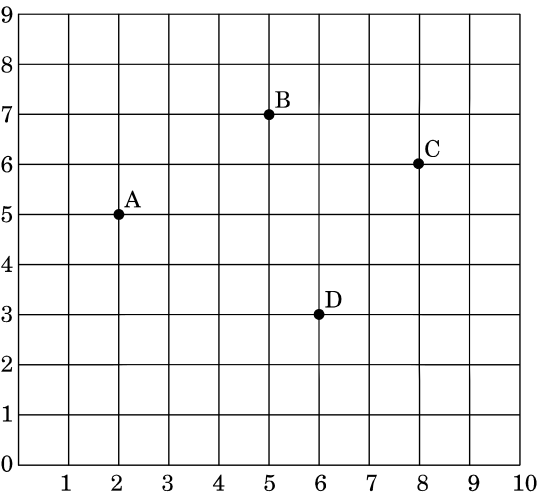
\includegraphics[width=0.5\textwidth,height=0.5\textwidth]{.\Figs\fig.png}
		     \caption{Based on the above, answer the following question :}
		     \label{fig:my_label}
	     \end{figure}
\begin{enumerate}[label=(\roman*)]
	\item The figure formed by the points $\vec{A}$, $\vec{B}$, $\vec{C}$ and $\vec{D}$ is a
		\begin{enumerate}[label=(\Alph*)]
			\item sqaure
			\item parallelogram
			\item rhombus
			\item quadrilateral
		\end{enumerate}
	\item If the sports teacher is sitting at the origin, then which of the four students is closest to him ?
		\begin{enumerate}[label=(\Alph*)]
			\item $\vec{A}$
			\item $\vec{B}$
			\item $\vec{C}$
			\item $\vec{D}$
		\end{enumerate}
	\item The distance between $\vec{A}$ and $\vec{C}$ is 
		\begin{enumerate}[label=(\Alph*)]
			\item $\sqrt{37}$ units
			\item $\sqrt{35}$ units
			\item $6$ units
			\item $5$ units
		\end{enumerate}
	\item The coordinates of the mid-point of line segment $AC$ are
	\item If a point $\vec{P}$ divides the line segment $AD$ in the ratio $1:2$, then coordinates of $\vec{P}$ are
		\begin{enumerate}[label=(\Alph*)]
			\item $(\frac{8}{3},\frac{8}{3})$
			\item $(\frac{10}{3},\frac{13}{3})$
			\item $(\frac{13}{3},\frac{10}{3})$
			\item $(\frac{16}{3},\frac{11}{3})$
	\end{enumerate}

\end{enumerate}
\item \begin{enumerate}[label=(\alph*)]
		\item Check whether the points $\vec{P}(5, -2)$, $\vec{Q}(6, 4)$ and $\vec{R}(7, -2)$ are the vertices of an isosceles triangle PQR.
		\item Find the ratio in which $\vec{P}(4, 5)$ divides the join of $\vec{A}(2, 3)$ and $\vec{B}(7, 8)$.
\end{enumerate}
\item The coordinate of the three consecutive vertices of a parallelogram ABCD are $\vec{A}(1, 3)$, $\vec{B}(-1, 2)$, and $\vec{C}(2, 5)$. Find the cordinates of the fourth vertex $\vec{D}$.

\item \begin{enumerate}[label=(\alph*)]
		\item If $\vec{P}(2, 2)$, $\vec{Q}(-4, -4)$ and $\vec{R}(5, -8)$ are the vertices of a $\triangle$PQR, then find the length of the median through $\vec{R}$.
		\item Find the ratio in which y-axis divides the line segment joining the points $\vec{A}(5, -6)$ and $\vec{B}(-1, -4)$.Also, find the coordinates of the point of intersection.
\end{enumerate}
\item
	\begin{enumerate}[label=(\alph*)]
		\item Find the ratio in which the line segment joining the points $\vec{A}(1, -5)$ and $\vec{B}(-4, 5)$ is divided by the ax-axis. Also, find coordinates of the point of division.
		\item The points $\vec{A}(0, 3)$, $\vec{B}(-2, a)$ and $\vec{C}(-1, 4)$ are the vertices of a rigth triangle, right-angled at $\vec{A}$. Find the value of a. 
	\end{enumerate}
\end{enumerate}
\end{document}
